\chapter{State of the art}

\section{Introduction}

I started my internship as web developer and tester focusing on how TDD and BDD can be introduced and used during the \textit{Bring The Food}\footnote{\url{http://www.bringfood.org}} development process. Bring The Food is a crowd-sourcing web and mobile application that allows people to fight food waste. From now, I will refer to Bring The Food only as the Ruby on Rails web application.

Ruby on Rails\footnote{\url{http://www.rubyonrails.org}} is an open-source web framework written in Ruby. It allows developers to build web pages and applications based on Ruby. Ruby on Rails emphasizes the use of well-known software engineering patterns and principles, such as active record pattern, don't repeat yourself (DRY), and model-view-controller (MVC). Rails was created in 2003 by David Heinemeier Hansson and has since been extended by the Rails core team and more than 3,400 contributors.

Ruby\footnote{\url{http://www.ruby-lang.org}} is an open source programming language developed in the mid-1990s by Yukihiro ``Matz'' Matsumoto. It supports multiple programming paradigms, including functional, object-oriented, and imperative. Bring The Food is written in Ruby 1.9.3, the same version that I used to develop \textit{Gherkin*} and \textit{Cucumber*}.

\section{Ruby and its approach to testing}

As \cite{book:villafiorita} states, a standard practice for project teams is to set up three exact and independent replicas of the same operating environment as follows.
\begin{itemize}
\item A \textbf{development environment} in which the development of applications take place. Developers usually use fancy data and work on them in order to make changes.
\item A \textbf{testing environment} in which testers test if the system in the development environment is ready to be deployed.
\item A \textbf{production environment} which is the version that final users use. Basically, when a new feature of an application is both developed and tested it will be deployed in this environment.
\end{itemize}

According to the official guide\footnote{\url{http://guides.rubyonrails.org/configuring.html}}, every Ruby on Rails web application has a test environment with which testers can use to execute test cases, without changing anything about the other two. Furthermore, since Ruby 1.8, a TDD framework is available in every Ruby project by default. In our case, Ruby 1.9.3 provides \textit{MiniTest}\footnote{\url{https://rubygems.org/gems/minitest}}, a complete suite of testing facilities supporting TDD and BDD, which allows developers to easily set up, organize and run tests. With it, tests for models and controllers may be easily written without other external tools.

However, its syntax is not easy to read and maintain over time. Fortunately, there are a various of frameworks available online. These frameworks are called gems and they can be either downloaded directly using the RubyGems packaging system\footnote{\url{https://rubygems.org}} or one of the world's largest code host: Github\footnote{\url{https://www.github.com}}. Gems help developers to build their web applications using facilities developed by other developers. In particular, there are some gems that help testers to write better tests. Most of the gems are released under the MIT License so, developers are free to use, copy, modify, or publish them. To solve the test code maintainability problem in Bring The Food we use \textit{RSpec} with \textit{Capybara}.

\section{RSpec and Capybara}

RSpec\footnote{\url{https://rubygems.org/gems/rspec}} is a BDD tool for Ruby programmers. It allows developers to write human readable specifications \cite{book:rspec}. This means that it provides a syntax closer to users by using pseudo natural language (e.g., RSpec uses words such as \textit{should} and \textit{expect} rather than \textit{assert}). Moreover, it takes a slightly different approach to the idea of testing applications, by testing ``behavior" rather than only specific methods \cite{intro_rspec}.

Capybara\footnote{\url{https://rubygems.org/gems/capybara}} helps testers to simulate how a real user would interact with them. For each test cases it opens an instance of a web browser and navigates between web pages. This gem is useful because with it testers are not only able to validate the behavior of web applications but also to test their graphic interface.

These gems help us to write tests more quickly than MiniTest. Thanks to Capybara, we write tests which cover also the front-end side of the application. 
However, RSpec has one important limit: while for the BDD technique, tests should be understood by stakeholders, RSpec mixes test description with test code, making difficult to read them. To solve this problem, we use other two Ruby gems which are of particular importance: \textit{Gherkin} and \textit{Cucumber}.

Gherkin and Cucumber are development tools that allow testers to write \textit{scenarios} \cite{book:cucumber}. They aims to bridge the gap between developers and stakeholders. These framework are both written in Ruby, but they can be used to test applications written either in Ruby or in other languages including Java, C\# and Python. The strength of those gems is that testers write scenarios in natural language without worrying about Ruby code. In fact, they overcomes the RSpec limit by separating test code from acceptance tests (scenarios).

\section{Gherkin}

Gherkin\footnote{\url{https://github.com/cucumber/gherkin}} is the core library of Cucumber. It allows us to define test cases that testers write in files with the \textit{.feature} extension. From now, these files will be called simply \textit{feature files}.

While all the scenarios are written in these files, test code is written in separated Ruby files, which contain blocks of code called \textit{step definitions}. These definitions are analogous to method definitions except one difference: their prototypes are defined by regular expressions.

The Gherkin gem allows Cucumber to parse feature files in order to execute all the scenarios written in them. An example of feature file taken from Bring The Food is shown in Figure \ref{figure:scenario_example_original}.

\begin{figure}[h!]
\begin{minted}[fontsize=\small,frame=single,linenos=true]{gherkin}
Feature: Login and logout as collector

  Scenario: Login
    Given I am on the login page
    When I sign in as "collector@example.com"
    Then I should see "Available Offers"

  Scenario: Logout
    Given I am logged in as "collector@example.com"
    When I sign out
    Then I should be redirected to the login page
\end{minted}
\vspace{-1em}
\caption{An example of a feature file taken from Bring The Food.}
\label{figure:scenario_example_original}
\end{figure}

As it can be seen, the syntax of feature files is really simple to understand since it uses a small set of keywords. As reported in the Cucumber Wiki\footnote{\url{https://github.com/cucumber/cucumber/wiki/Feature-Introduction}}, most lines in them start with one of the special keyword written in Table \ref{table:gherkin_keywords}.

\begin{table}[h!]
	\vspace{0.2cm}
	\renewcommand*\arraystretch{1.5}
	\begin{center}
	\textit{ 
		\begin{tabular}{|cccc|}
			\hline
			\multicolumn{4}{|c|}{Scenario Outline} \\
			Name & Native & Encoding & Scenario \\
			Feature & Background & Examples & Given \\
			When & Then & And & But \\ \hline
		\end{tabular}
	}
	\caption{The set of Gherkin's keywords.}
	\label{table:gherkin_keywords}
	\vspace{-1.2em}
	\end{center}
\end{table}

These keywords are used by testers during test cases definitions. In other words, testers combine keywords such as \textit{Feature} and \textit{Scenario} to define specifications for each new feature and new scenario to develop.

Every feature file consists of one single feature. In order to define a new feature, testers write the keyword \textit{Feature} followed by a plain-text description. After the description, other text may be written in order to describe which tests will be covered in that feature. Each feature usually contains a list of scenarios, so testers may add the keyword \textit{Scenario} on a new line. The text immediately following on the same line as the Scenario keyword is the name of the scenario. Each scenario contains a list of steps, each of these is composed by a sentence which must start by one of the words \textit{Given}, \textit{When}, \textit{Then}, \textit{And} and \textit{But}. For Cucumber there are no differences between the previous keywords: all of them are treated as the same. However, those words should help testers to write descriptive test cases following the natural language. So, while the word ``Given'' should represent an initial condition, the word ``When'' should be interpreted as an action and the word ``Then'' should be considered as an expected result. The conjunctions ``And'' and ``But'' are usually used in case of multiple conditions, actions or results. 

In addition to being a library, Gherkin defines the language that Cucumber understands. Consequently, its grammar defines how feature files must be written correctly.

To allow Cucumber to parse feature files, Gherkin defines a lexer using Ragel\footnote{\url{http://www.complang.org/ragel}}, which is a lexer generator that allows users to define a lexer starting from regular expressions.
The lexer is written starting from the grammar, which is defined by productions written as regular expressions in a bottom-up notation. The flow is the following: Gherkin uses the grammar's file as input to Ragel which compiles it into a Finite State Machine (FSM) and produces the final lexer as output in a Ruby file. Afterwards, the parser uses a parsing table to check if a feature file is syntactically correct. Table \ref{table:parsing_table_gherkin} shows the parsing table used by Gherkin. As can be seen, most of the cells in the table contain the Expected Error (E) value. The parser occurs these cells when a file violates a rule of the language. In this case, a parsing error is raised and the parsing process is stopped.

\begin{table}[h!]
	\renewcommand*\arraystretch{1.5}
	\centering
	\resizebox{\linewidth}{!}{
	\begin{tabular}{|r|l|l|l|l|l|l|l|l|l|l|l|l|}
	\cline{2-10}
	\multicolumn{1}{r|}{} 	& feature & background & scenario      & scenario\_outline 	& examples & step         	& row            	& doc\_string   	& eof \\ \hline
	root             		& feature & E          & E             & E                	& E        & E            	& E              	& E            		& eof \\ \hline
	feature          		& E       & background & scenario      & scenario\_outline 	& E        & E            	& E              	& E            		& eof \\ \hline
	step             		& E       & E          & scenario      & scenario\_outline 	& E        & step         	& step           	& step         		& eof \\ \hline
	outline\_step    		& E       & E          & scenario      & scenario\_outline 	& examples & outline\_step 	& outline\_step   	& outline\_step 	& eof \\ \hline
	background       		& E       & E          & scenario      & scenario\_outline 	& E        & step         	& E              	& E            		& eof \\ \hline
	scenario         		& E       & E          & scenario      & scenario\_outline 	& E        & step         	& E              	& E            		& eof \\ \hline
	scenario\_outline 		& E       & E          & E             & E                	& E        & outline\_step 	& E              	& E            		& eof \\ \hline
	examples        		& E       & E          & E             & E                	& E        & E            	& examples\_table 	& E            		& eof \\ \hline
	examples\_table   		& E       & E          & scenario      & scenario\_outline 	& examples & E            	& examples\_table 	& E            		& eof \\ \hline
	eof              		& E       & E          & E             & E                	& E        & E            	& E              	& E            		& E   \\ \hline
	\end{tabular}
	}
	\caption{The parsing table used by Gherkin to parse feature files.}
	\label{table:parsing_table_gherkin}
\end{table}

Consider now that some keywords shown in Table \ref{table:gherkin_keywords} are not used for defining test cases. Moreover, even though there are slight differences between \textit{Scenario} and \textit{Scenario Outline}\footnote{\url{https://github.com/cucumber/cucumber/wiki/Scenario-Outlines}}, both keywords define a test case. Hence, we can focus on the first word, and in particular on a set of keywords which is smaller than the original one.
\[
\Set{Feature, Background, Scenario, Given, When, Then, And, But}
\]
The set defined above includes all the keywords that can be used by testers in order to define test cases. The keyword \textit{Background}, is used to define conditions that must be satisfied at the beginning of each scenarios written in the same file. Since all the step keywords \textit{Given}, \textit{When}, \textit{Then}, \textit{And} and \textit{But} are treated as the same by Cucumber, we can group all of them in one set we call Step, obtaining the following result.
\[
\Set{Feature, Background, Scenario, Step}
\]
Figure \ref{figure:automaton} shows part of the FSM produced by Ragel. In that automaton, all the states are necessary to parse feature files composed by the keywords above. The same automaton can be obtained considering Table \ref{table:parsing_table_gherkin} as follows: while the first column contains all the states of the automaton, the first row shows all the possible tokens that can be recognized by the parser and the remaining cells are transitions between states. There is an initial state \textit{root} and a final state \textit{eof}. All the transitions that outcome or move back to the E state are not considered.
A feature file is correct only if the parser arrives in the eof state once that the file is completely parsed. For instance, if we consider the \textit{Feature} state we can note that there are three transitions outcome from it. These transitions are allowed because after a \textit{Feature} definition, testers may define either a new \textit{Scenario} or a \textit{Background} definition. However, they can not define directly a step definition because steps must be defined within a \textit{Scenario} or a \textit{Background}.

\begin{figure}[H]
	\centering
	\begin{tikzpicture}[scale=0.14]
	\tiny{
	\tikzstyle{every node}+=[inner sep=0pt]
	\draw [black] (5.2,-29) circle (3);
	\draw (5.2,-29) node {$root$};
	\draw [black] (22.6,-29) circle (3);
	\draw (22.6,-29) node {$feature$};
	\draw [black] (42.8,-29) circle (3);
	\draw (42.8,-29) node {$\substack{back\\ground}$};
	\draw [black] (42.8,-48.1) circle (3);
	\draw (42.8,-48.1) node {$eof$};
	\draw [black] (42.8,-48.1) circle (2.4);
	\draw [black] (42.8,-9.9) circle (3);
	\draw (42.8,-9.9) node {$\substack{sce\\nario}$};
	\draw [black] (62.9,-29) circle (3);
	\draw (62.9,-29) node {$step$};
	\draw [black] (8.2,-29) -- (19.6,-29);
	\fill [black] (19.6,-29) -- (18.8,-28.5) -- (18.8,-29.5);
	\draw (13.9,-28.5) node [above] {$feature$};
	\draw [black] (7.87,-30.36) -- (40.13,-46.74);
	\fill [black] (40.13,-46.74) -- (39.64,-45.93) -- (39.19,-46.82);
	\draw (22.24,-39.06) node [below] {$eof$};
	\draw [black] (24.78,-31.06) -- (40.62,-46.04);
	\fill [black] (40.62,-46.04) -- (40.38,-45.13) -- (39.7,-45.85);
	\draw (34.49,-38.07) node [above] {$eof$};
	\draw [black] (25.6,-29) -- (39.8,-29);
	\fill [black] (39.8,-29) -- (39,-28.5) -- (39,-29.5);
	\draw (32.7,-29.5) node [below] {$background$};
	\draw [black] (24.78,-26.94) -- (40.62,-11.96);
	\fill [black] (40.62,-11.96) -- (39.7,-12.15) -- (40.38,-12.87);
	\draw (28.85,-18.97) node [above] {$scenario$};
	\draw [black] (45.421,-11.359) arc (59.16523:33.75739:49.833);
	\fill [black] (45.42,-11.36) -- (45.85,-12.2) -- (46.36,-11.34);
	\draw (58.05,-17.54) node [above] {$scenario$};
	\draw [black] (65.58,-27.677) arc (144:-144:2.25);
	\draw (70.15,-29) node [right] {$step$};
	\fill [black] (65.58,-30.32) -- (65.93,-31.2) -- (66.52,-30.39);
	\draw [black] (41.477,-7.22) arc (234:-54:2.25);
	\draw (42.8,-2.65) node [above] {$scenario$};
	\fill [black] (44.12,-7.22) -- (45,-6.87) -- (44.19,-6.28);
	\draw [black] (42.8,-26) -- (42.8,-12.9);
	\fill [black] (42.8,-12.9) -- (42.3,-13.7) -- (43.3,-13.7);
	\draw (42.3,-19.45) node [left] {$scenario$};
	\draw [black] (45.8,-29) -- (59.9,-29);
	\fill [black] (59.9,-29) -- (59.1,-28.5) -- (59.1,-29.5);
	\draw (52.85,-29.5) node [below] {$step$};
	\draw [black] (60.344,-27.43) arc (-123.00486:-144.07252:59.783);
	\fill [black] (60.34,-27.43) -- (59.95,-26.57) -- (59.4,-27.41);
	\draw (49.6,-21.11) node [below] {$step$};
	\draw [black] (60.73,-31.07) -- (44.97,-46.03);
	\fill [black] (44.97,-46.03) -- (45.9,-45.84) -- (45.21,-45.12);
	\draw (54.64,-39.03) node [below] {$eof$};
	\draw [black] (45.537,-8.677) arc (110.11043:-110.11043:21.643);
	\fill [black] (45.54,-49.32) -- (46.12,-50.07) -- (46.46,-49.13);
	\draw (75.12,-29) node [right] {$eof$};
	\draw [black] (42.8,-32) -- (42.8,-45.1);
	\fill [black] (42.8,-45.1) -- (43.3,-44.3) -- (42.3,-44.3);
	\draw (43.3,-38.55) node [right] {$eof$};
	\draw [black] (1.2,-25.2) -- (3.03,-26.93);
	\fill [black] (3.03,-26.93) -- (2.79,-26.02) -- (2.1,-26.75);
	}
	\end{tikzpicture}
	\caption{The FSM built by Ragel.}
	\label{figure:automaton}
\end{figure}

Consider now, that every state in the automaton shown in Figure \ref{figure:automaton} has a transition that goes to the final state. Hence, we can reduce the graph removing the \textit{eof} state and converting all the states in finals. The result can be seen in Figure \ref{figure:gherkin_fsm_simple}.

\begin{figure}[h!]
	\centering
	\tiny{
	\begin{tikzpicture}[scale=0.15]
	\tikzstyle{every node}+=[inner sep=0pt]
	\draw [black] (5.2,-29) circle (3);
	\draw (5.2,-29) node {$root$};
	\draw [black] (5.2,-29) circle (2.4);
	\draw [black] (22.6,-29) circle (3);
	\draw (22.6,-29) node {$feature$};
	\draw [black] (22.6,-29) circle (2.4);
	\draw [black] (45.1,-29) circle (3);
	\draw (45.1,-29) node {$\substack{back\\ground}$};
	\draw [black] (45.1,-29) circle (2.4);
	\draw [black] (45.1,-9.9) circle (3);
	\draw (45.1,-9.9) node {$\substack{sce\\nario}$};
	\draw [black] (45.1,-9.9) circle (2.4);
	\draw [black] (68.1,-29) circle (3);
	\draw (68.1,-29) node {$step$};
	\draw [black] (68.1,-29) circle (2.4);
	\draw [black] (8.2,-29) -- (19.6,-29);
	\fill [black] (19.6,-29) -- (18.8,-28.5) -- (18.8,-29.5);
	\draw (13.9,-28.5) node [above] {$feature$};
	\draw [black] (25.6,-29) -- (42.1,-29);
	\fill [black] (42.1,-29) -- (41.3,-28.5) -- (41.3,-29.5);
	\draw (33.85,-29.5) node [below] {$background$};
	\draw [black] (24.89,-27.06) -- (42.81,-11.84);
	\fill [black] (42.81,-11.84) -- (41.88,-11.98) -- (42.53,-12.74);
	\draw (30.01,-18.96) node [above] {$scenario$};
	\draw [black] (47.791,-11.224) arc (62.31309:38.27207:57.772);
	\fill [black] (47.79,-11.22) -- (48.27,-12.04) -- (48.73,-11.15);
	\draw (61.7,-17.44) node [above] {$scenario$};
	\draw [black] (70.78,-27.677) arc (144:-144:2.25);
	\draw (75.35,-29) node [right] {$step$};
	\fill [black] (70.78,-30.32) -- (71.13,-31.2) -- (71.72,-30.39);
	\draw [black] (43.777,-7.22) arc (234:-54:2.25);
	\draw (45.1,-2.65) node [above] {$scenario$};
	\fill [black] (46.42,-7.22) -- (47.3,-6.87) -- (46.49,-6.28);
	\draw [black] (45.1,-26) -- (45.1,-12.9);
	\fill [black] (45.1,-12.9) -- (44.6,-13.7) -- (45.6,-13.7);
	\draw (44.6,-19.45) node [left] {$scenario$};
	\draw [black] (48.1,-29) -- (65.1,-29);
	\fill [black] (65.1,-29) -- (64.3,-28.5) -- (64.3,-29.5);
	\draw (56.6,-29.5) node [below] {$step$};
	\draw [black] (65.464,-27.569) arc (-119.74114:-139.6737:69.37);
	\fill [black] (65.46,-27.57) -- (65.02,-26.74) -- (64.52,-27.61);
	\draw (53.44,-21.2) node [below] {$step$};
	\draw [black] (1.2,-25.2) -- (3.03,-26.93);
	\fill [black] (3.03,-26.93) -- (2.79,-26.02) -- (2.1,-26.75);
	\end{tikzpicture}
	}
	\caption{A simplified version of the FSM built by Ragel.}
	\label{figure:gherkin_fsm_simple}
	\vspace{0.2cm}
\end{figure}

While the parsing process is running, the parser sends an event to a Cucumber listener which executes semantic actions for each keyword found.

\newpage
\section{Cucumber}

Cucumber\footnote{\url{https://github.com/cucumber/cucumber}} uses Gherkin to parse feature files in order to execute all the scenarios.

Every time that the Gherkin's parser finds a keyword, it sends to the Cucumber listener that word followed by the plain-text written until the next keyword. This mechanism is made possible because keywords are always followed by plain text (i.e, see Figure \ref{figure:scenario_example_original}). When these values are received by the listener, Cucumber runs a semantic action associated to that keyword. Basically, these actions are functions that build an Abstract Syntax Tree (AST) for each feature file analysed. In particular, every node in the tree has the structure illustrated by Figure \ref{table:node_structure}.

\begin{table}[h!]
	\renewcommand*\arraystretch{1.3}
	\begin{center}
	\begin{tabular}{|c|c|}
		\hline
		\multicolumn{2}{|c|}{\textit{parent}} \\ \hline
		\textit{keyword} & \textit{plaintext} \\ \hline
		\multicolumn{2}{|c|}{$child_1$ ... $child_n$} \\ \hline
	\end{tabular}
	\caption{The structure of nodes in the AST built by Cucumber.}
	\label{table:node_structure}
	\end{center}
\end{table}

The tree is built as following: when the keyword \textit{Feature} is recognized by Gherkin, a new instance of an AST is created and a new node composed by the word Feature and its description is added as root to that tree.
When the word recognized is \textit{Scenario}, a new child node is added to the root node. This node will contain the values Scenario as keyword and the name of the scenario as plain-text. The same process happens when a step keywords is found: all the steps of a scenario becomes children nodes of that scenario node. Steps will be leaf nodes of the tree.

Figure \ref{figure:ast_cucumber} shows the AST built by Cucumber for the feature file shown in Figure \ref{figure:scenario_example_original}.

\begin{figure}[H]
	\centering
	\synttree	[Feature
			    	[Login
				    	[$Step_i$]
				    	[\dots]
				    	[$Step_n$]
					]
			    	[Logout
			    		[$Step_k$]
			    		[\dots]
			       		[$Step_m$]
					]
				]
	\vspace{0.2cm}
	\caption{An example of an Abstract Syntax Tree built by Cucumber.}
	\label{figure:ast_cucumber}
\end{figure}

In the end of the parsing process, Cucumber has an AST instance with the same structure of the feature file parsed.

To execute all the scenarios stored in the AST, Cucumber creates an instance of a \textit{Visitor} class which starts a preorder tree traversal. Each scenario is executed as a separate test case, with no interaction to other scenarios or features. The output produced by Cucumber is the following:

\begin{itemize}
\item If the node visited has the words Feature or Scenarios in the keyword field, the output is the keyword followed by the plain-text as written in the input file.
\item If the node visited has a step keyword in the keyword field, Cucumber tries to match the plain-text with a regular expression written in a step definition file. If a match is found then the test code written into that step definition is executed, otherwise a pending error is raised and the execution is stopped.
\end{itemize}

Cucumber also formats the output on the terminal providing indentation and displaying each step with a color: passing steps are coloured green, failing steps red, and undefined and pending steps yellow. When a step fails or is undefined, Cucumber skips to the next scenario and colors the skipped steps cyan\footnote{\url{https://github.com/cucumber/cucumber/wiki/Step-Definitions}}.

The output of the Cucumber execution of the feature file visible in Figure \ref{figure:scenario_example_original} can be seen in Figure \ref{figure:scenario_example_original_executed}. 

\begin{figure}[h!]
\begin{minted}[fontsize=\small,frame=single]{gherkin}
Feature: Login and logout as collector

  Scenario: Login
    Given I am on the login page
    When I sign in as "collector@example.com"
    Then I should see "Available Offers"

  Scenario: Logout
    Given I am logged in as "collector@example.com"
    When I sign out
    Then I should be redirected to the login page

2 scenarios (2 passed)
6 steps (6 passed)
0m0.010s
\end{minted}
\vspace{-1em}
\caption{The result of the execution of Cucumber.}
\label{figure:scenario_example_original_executed}
\end{figure}

\newpage
\section{SimpleCov}

To gather information about our tests in Bring The Food we use a code coverage analysis tool for Ruby called \textit{SimpleCov}\footnote{\url{https://rubygems.org/gems/simplecov}}. SimpleCov gathers code coverage data from all tests including Cucumber's step definitions, RSpec and Capybara. It analyses which lines of code are covered by tests and then formats the results providing an html output file where the percentage of code coverage can be seen for each Ruby file in the project. We can also see the coverage for categories such as controllers, models, mailers and helpers.

The first time we used SimpleCov in Bring the Food we got the 50\% of code coverage. This result was expected considering the following aspects:

\begin{enumerate}
\item We tested only the main features of the application including the Sign up, the Login, the Logout and other actions such as publishing, booking, editing and deleting food donations.
\item We introduced the BDD technique when most of the application's features were already developed.
\end{enumerate}

If we consider the results provided by this tool, we may infer that the 50\% of our application has been tested.
Unfortunately, in a high-level language like Ruby, some lines of code marked as covered by SimpleCov, may not be tested by test cases. In fact, some of these are marked simply by loading the test environment.

\section{Gems overview}

All the previous gems can be combined in order to enforce the validation of Ruby on Rails web applications.

\begin{table}[h!]
	\vspace{0.2cm}
	\renewcommand*\arraystretch{1.5}
	\begin{center}
	\begin{tabular}{|c|}
		\hline
		SimpleCov \\ \hline
		Gherkin and Cucumber \\ \hline
		RSpec and Capybara \\ \hline
		MiniTest \\ \hline
	\end{tabular}
	\vspace{0.2cm}
	\caption{The BDD gem stack used in Bring The Food.}
	\label{table:structureofgems}
	\end{center}
\end{table}

Table \ref{table:structureofgems} shows how I used those gems: starting from the bottom, where the default MiniTest framework can be seen, going up to the last gem introduced in the Bring The Food development process.

